\originalchapter{习题课三: 高斯定律}
题源为\href{https://ocw.mit.edu/courses/8-02-physics-ii-electricity-and-magnetism-spring-2007/resources/solving03/}{Problem Solving 3}, PDF第1--6页. 原件主情境包含步骤1--8(步骤7有两问)和两势差问, 另有考试练习题. 所有解答为AI独立解答.

\begin{exercise}
半径$a$、长$L$的实心绝缘圆柱内均匀分布$+Q$, 外有半径$b>a$、同长的很薄绝缘圆柱壳均匀带$-Q$. $a<r<b$是真空. 采用足够长且远离端部的近似. 依原件顺序回答:
\begin{enumerate}
\item 步骤1: 指出对称性.
\item 步骤2: 指出场方向.
\item 步骤3: 空间分为几个场公式区域?
\item 步骤4: 每区选什么高斯面、以什么变量参数化、变量范围是什么?
\item 步骤5: 对$r<a$写含未知场的通量.
\item 步骤6: 对$r<a$用$Q,r,a$写包围电荷(必要时含高斯面长度与$L$).
\item 步骤7 Q1: 用通量等式求$r<a$场; Q2: 对$a<r<b$重复.
\item 步骤8: 画各区场大小图, 包括$r>b$.
\item 倒数第二问: 求$V(a)-V(0)$.
\item 最后一问: 求$V(b)-V(a)$.
\end{enumerate}
\end{exercise}
\begin{solution}
1--2. 近似轴向平移、绕轴旋转和轴向反射对称, 场径向, 正柱外指向外.
3--4. 三个区域$r<a,a<r<b,r>b$, 以半径$r$同轴高斯柱、长度$h$作面; 两端无通量, 侧面等大且法向.
5. 通量$2\pi rhE(r)$.
6. 密度$\rho=Q/(\pi a^2L)$, 包围电荷$\rho\pi r^2h=Qhr^2/(La^2)$; 若取$h=L$便为$Qr^2/a^2$, 但长柱近似仍要求远离真实端部.
7--8. 将包围量代入, 得
\[
E(r)=\frac Q{2\pi\eps L}\begin{cases}r/a^2,&0\le r<a,\\1/r,&a<r<b,\\0,&r>b.\end{cases}
\]
外区包围净电荷为零且有柱对称, 所以场零. 在$a$两侧连续, 在$b$带面电荷处由内侧有限值跳到零.
9. $V(a)-V(0)=-\int_0^a Qr\dd r/(2\pi\eps La^2)=-Q/(4\pi\eps L)$.
10. $V(b)-V(a)=-Q\ln(b/a)/(2\pi\eps L)$.
\begin{center}
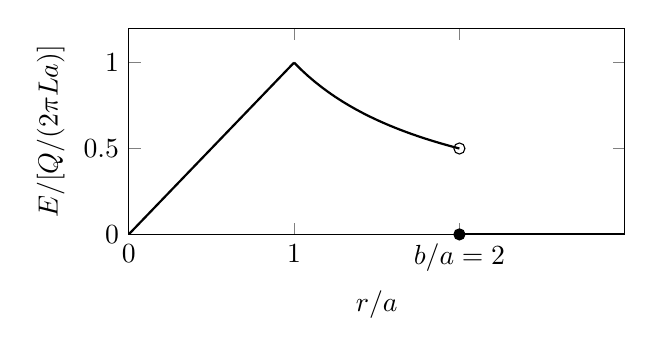
\begin{tikzpicture}
\begin{axis}[width=.65\linewidth,height=4.2cm,xlabel={$r/a$},ylabel={$E/[Q/(2\pi\eps La)]$},xmin=0,xmax=3,ymin=0,ymax=1.2,xtick={0,1,2},xticklabels={0,1,$b/a=2$},ytick={0,.5,1}]
\addplot[domain=0:1,thick] {x};\addplot[domain=1:2,thick] {1/x};\addplot[domain=2:3,thick] {0};
\addplot[only marks,mark=o] coordinates {(2,.5)};\addplot[only marks] coordinates {(2,0)};
\end{axis}
\end{tikzpicture}
\end{center}
图用$b/a=2$示意, 非原题指定数值. 跃变点的理想面上场不作为单侧有限值来定义.
\end{solution}

\begin{exercise}
考试练习题. 电荷厚板在$y,z$方向无限, $-1\,\mathrm m<x<1\,\mathrm m$内有均匀体密度$\rho$. 原图电势在两侧为与内部光滑连接的直线, 内部为$V(x)=(15\,\mathrm{V/m^2})x^2/2-25\,\mathrm V/2$. 求(a)左侧$E_x$; (b)右侧$E_x$; (c)板内$E_x$; (d)利用高斯定律求$\rho$.
\end{exercise}
\begin{solution}
(c)$E_x=-\dd V/\dd x=-(15\,\mathrm{V/m^2})x$. 原图两侧直线在边界的斜率与内部连接且无额外面电荷, 所以(a)$E_x=+15\,\mathrm{V/m}$, (b)$E_x=-15\,\mathrm{V/m}$. (d)取板内对称扁柱, $2E_x(x)A=\rho(2xA)/\eps$, 得$\rho=-15\eps\,\mathrm{V/m^2}\simeq-1.33\times10^{-10}\,\mathrm{C/m^3}$. 原图是势的谷, 对应负体电荷, 不能因题名“带电板”便假定$\rho>0$.
\end{solution}
